\section{The Problem to Solve}
\subsection{The Problem in its Entirety}
Starting from audio recordings of DTMF codes (explained below), the objective will be to distinguish the number of the pressed key based on the recording.

\subsection{What is DTMF Code?}
A DTMF code is a combination of frequencies used for traditional telephony. The frequencies used are specified in the table below. These codes are emitted when a key on the telephone keypad is pressed, resulting in a distinct sound produced for each key.

\begin{figure}[H]
\begin{center}
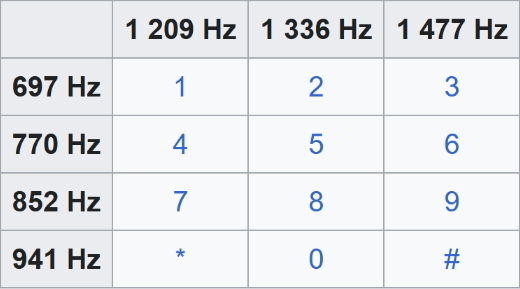
\includegraphics[height=5cm]{img/fig.jpg}\\
\caption{The frequency table associated with each button}
\end{center}
\end{figure}

\subsection{What is an Audio Recording?}
We will be provided with an audio recording that corresponds to the evolution of the amplitude of the sound signal over time.
